\section{Physics Baseline and Outcomes}
\label{sec:physics}

\subsection{What physics predicts}
For a
near-circular orbit, drag shrinks the semi-major axis $a$ at the rate
\begin{equation}
\frac{da}{dt} = -B\,\rho\,\sqrt{\mu a}, \qquad B = \frac{C_D A}{m},
\label{eq:drag}
\end{equation}
where $\rho$ is the neutral mass density, $\mu$ is Earth's gravitational parameter and $B$ is
the object's drag sensitivity (m$^2$/kg). For every interval we propagate the orbit with SGP4 at
evenly spaced times, half from each end's TLE, and look up $\rho$ along the track with
NRLMSIS~2.1~\cite{emmert2022msis21}, using NRLMSISE-00~\cite{picone2002nrlmsise} as a robustness
check. The model is driven by the observed F10.7, its 81-day mean and the 3-hourly ap history.
The interval's density driver is $D = -\overline{\rho\sqrt{\mu a}}$, and the predicted decay is
$B\,D$.

We do not take $B$ from a catalogue. Instead we fit it for each object on quiet intervals away
from any storm, as a $\Delta t$-weighted ratio of sums,
$\hat B = \sum_i \dot a_i \Delta t_i / \sum_i D_i \Delta t_i$, using every other quiet interval
and holding the rest back for validation. Before the fit, a Hampel filter on the residual
(five-day window, $k=3.5$) removes bad TLE pairs. A weekly block bootstrap puts the median
standard error of $\hat B$ at 3\% (maximum 8\%), and no object breaks the instability rule we
set in advance (fewer than 30 fit intervals, a standard error above 25\% of $\hat B$, or an
interval reaching zero).

\subsection{Two outcomes}
From the same observed decay $\dot a^{\text{obs}}$ we build two outcomes, both in m/day:
\begin{align}
Y_{\text{total}} &= \dot a^{\text{obs}} - \hat B\,D(\text{F10.7},\,ap_{\text{quiet}}),\\
Y_{\text{residual}} &= \dot a^{\text{obs}} - \hat B\,D(\text{F10.7},\,ap).
\end{align}
$Y_{\text{total}}$ runs the model with ap held at the storm's pre-storm quiet value (the median
ap over days $-10$ to $-3$). It asks what the storm did beyond a calm atmosphere, so it measures
the \emph{total storm effect}, and it is the outcome we read causally. $Y_{\text{residual}}$ uses
the real ap, so it asks what NRLMSIS~2.1 missed and measures the \emph{model error}. Strictly,
it also soaks up any storm-time change in the drag coefficient and any leftover TLE artifacts,
so it is model error in that broad sense. In both outcomes F10.7 stays at its real value, so the
baseline already accounts for UV before any statistics, and negative values mean more decay
than the baseline. Air density sits on the path from storm to decay
(storm $\rightarrow$ density $\rightarrow$ drag), so it enters only through this baseline and is
never used as a control.

\subsection{Does the baseline work?}
On the 50,674 held-out quiet intervals the mean NRLMSIS~2.1 residual is $-0.13$~m/day, with a
weekly-block standard error of 1.07~m/day, against a mean decay of $-50.6$~m/day. The per-object $t$-statistics have a
standard deviation of 0.82, and 6 of 250 objects have $|t|>2$, about what chance alone would
give. For the 116 rocket bodies with a DISCOSweb mass and cross-section, our fitted $\hat B$
ranks the objects the same way as the catalogue value $2.2\,A/m$ (Spearman $\rho = 0.81$,
Fig.~\ref{fig:valid}). These bodies come from about 15 stage types, so this is really a check
on stage types, not on 116 independent points. Fitted $\hat B$ is about 0.8 times the catalogue
value, which fits an orientation-averaged cross-section, so we only use the ranking as
validation.

\begin{figure}[t]
\centering
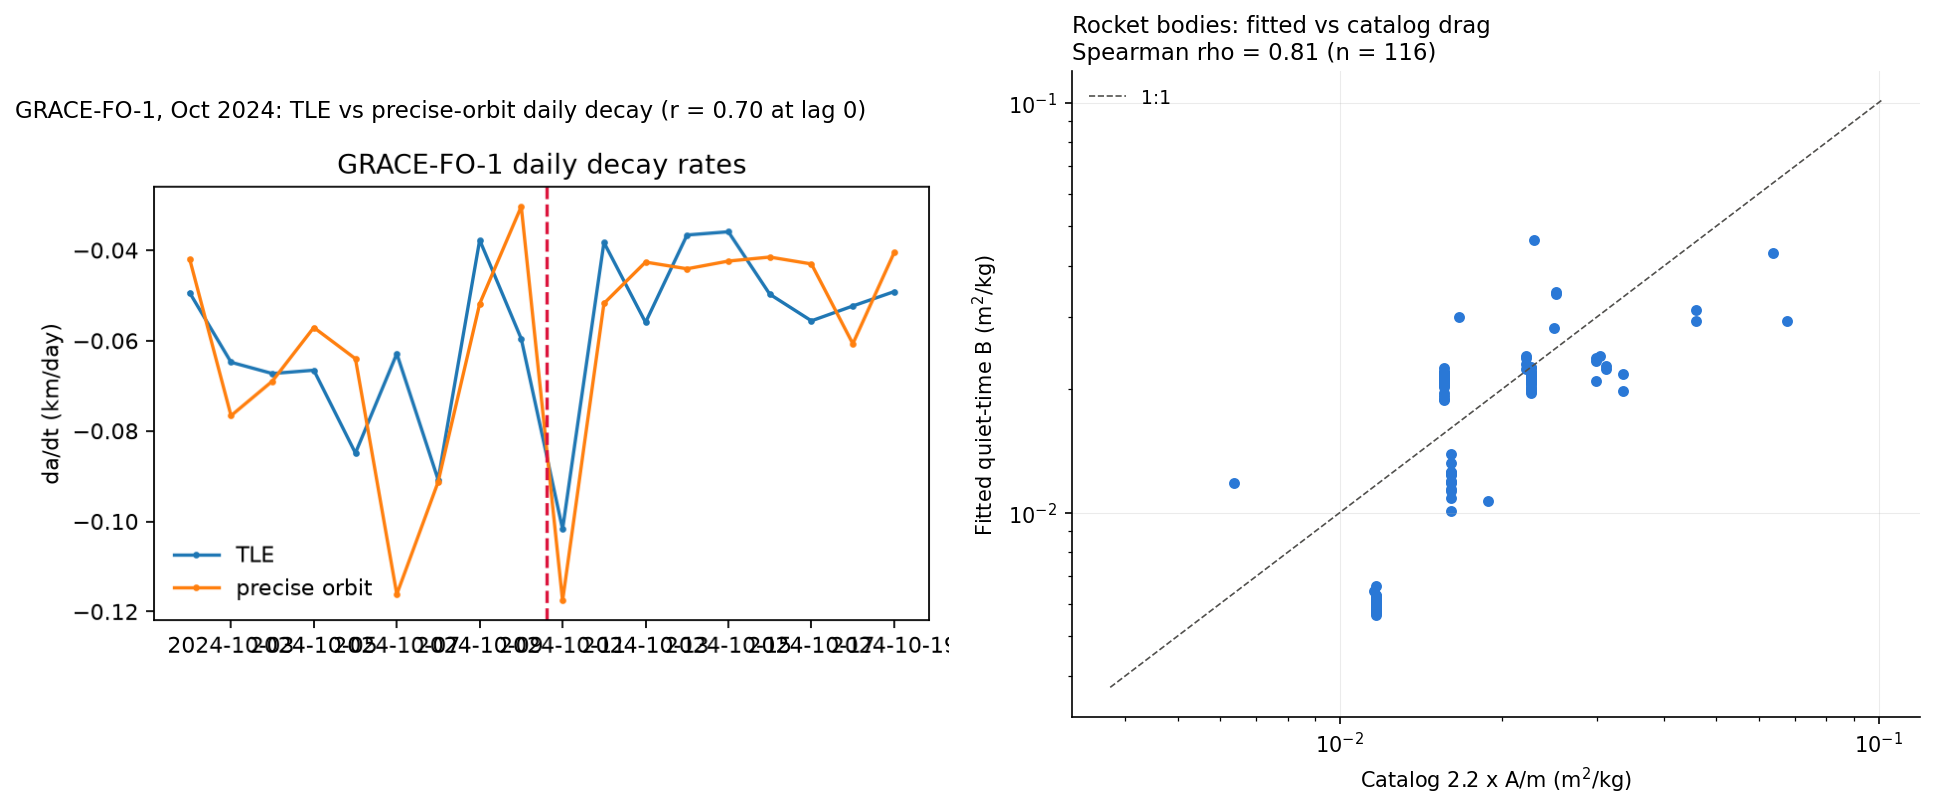
\includegraphics[width=\columnwidth]{fig6_validation.png}
\caption{Validation. Left: TLE-derived and precise-orbit decay rates of GRACE-FO-1 in October
2024 ($r=0.70$ at zero lag). Right: fitted drag sensitivity against the catalogue value for 116
rocket bodies (Spearman $\rho=0.81$).}
\label{fig:valid}
\end{figure}

\subsection{A simulator with a known answer}
We also built a simulator that integrates
Eq.~\eqref{eq:drag} through NRLMSIS~2.1 density for synthetic objects at 400--800~km. It plants
a storm boost of known size (by default $+50\%$ on days 0--2, gone by day 5), adds TLE-style
noise that triples during storms, and then runs everything through the same cleaning, fitting
and estimation code as the real data. With no noise the prediction follows the truth (median
error below 1\%), with no boost the residual is zero, and the planted boost is recovered inside
the event-study 95\% interval.
